\chapter{Local structure of LSCO+O due to interstitial oxygen (PDF, XAS)}

\begin{framed}
	\begin{itemize}
		\item PDF measurements. Presentation of data. Extraction of distributions (Cu-Oeq).
		\item Superstructure single-crystal measurements
		\item Comparison with simulation.
		\item Why is this structural problem hard? Is it important?
		\item Discussion: Is this impossible to explain with relatively small simulation cells?
		\item Outlook: Classical MD/RMC?
	\end{itemize}
\end{framed}

\section{Data}

\begin{figure}[H]
    \centering
    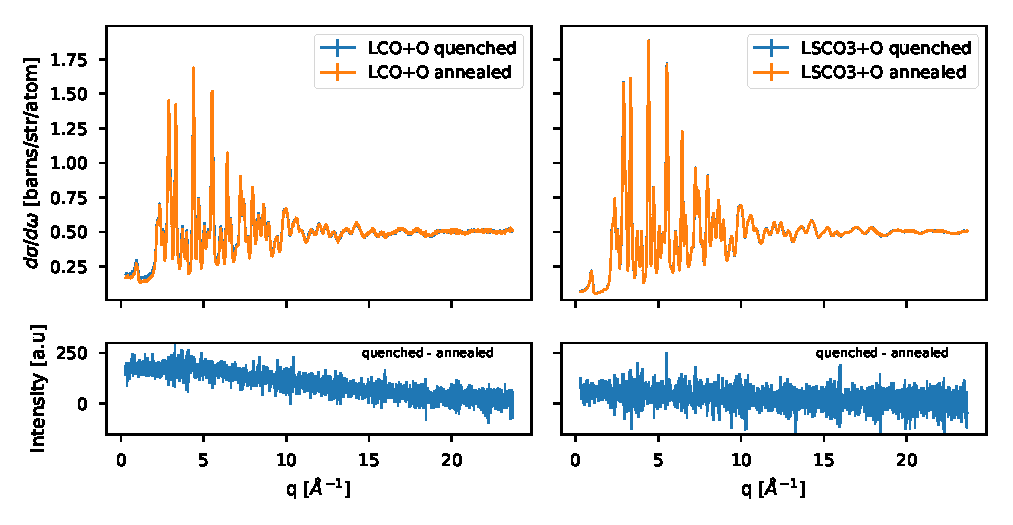
\includegraphics[width=\textwidth]{fig/pdf/quenched_annealed.pdf}
    \caption{Difference between quenched and annealed cooling procedures for LCO+O and LSCO3+O samples. The topmost plots are comparisons of the reduced and corrected $\text{d}\sigma/\text{d}\omega$ in absolute units, while the difference curves are extracted from the raw $\bm{q}$ data.}
    \label{fig:difference}
\end{figure}

\begin{figure}[H]
    \centering
    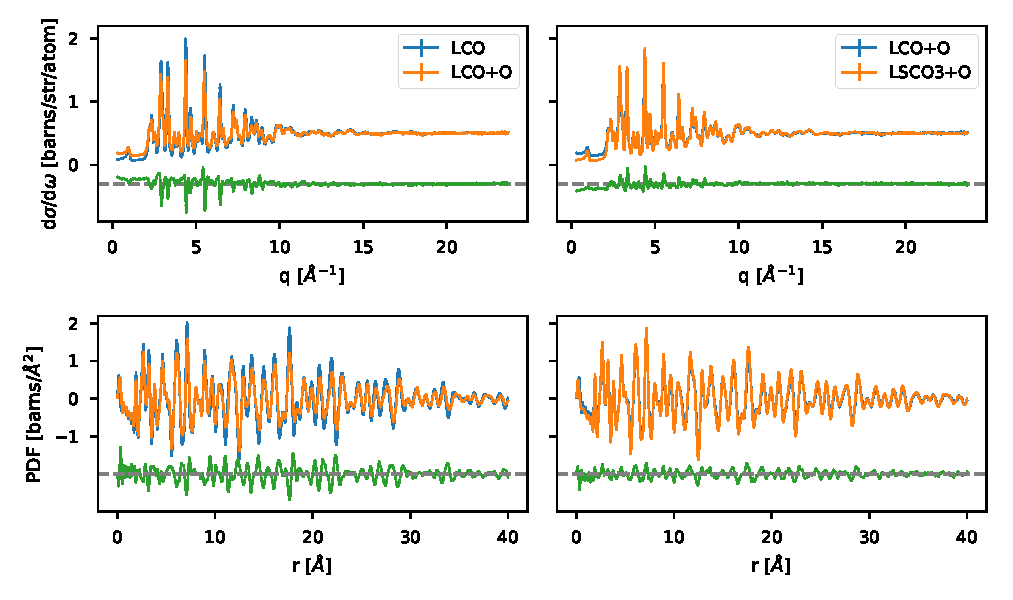
\includegraphics[width=\textwidth]{fig/pdf/sample_comparison.pdf}
    \caption{Comparison of the different samples at \SI{300}{\kelvin} in both real and reciprocal space.}
    \label{fig:sample_comparision}    
\end{figure}

\begin{figure}[H]
    \centering
    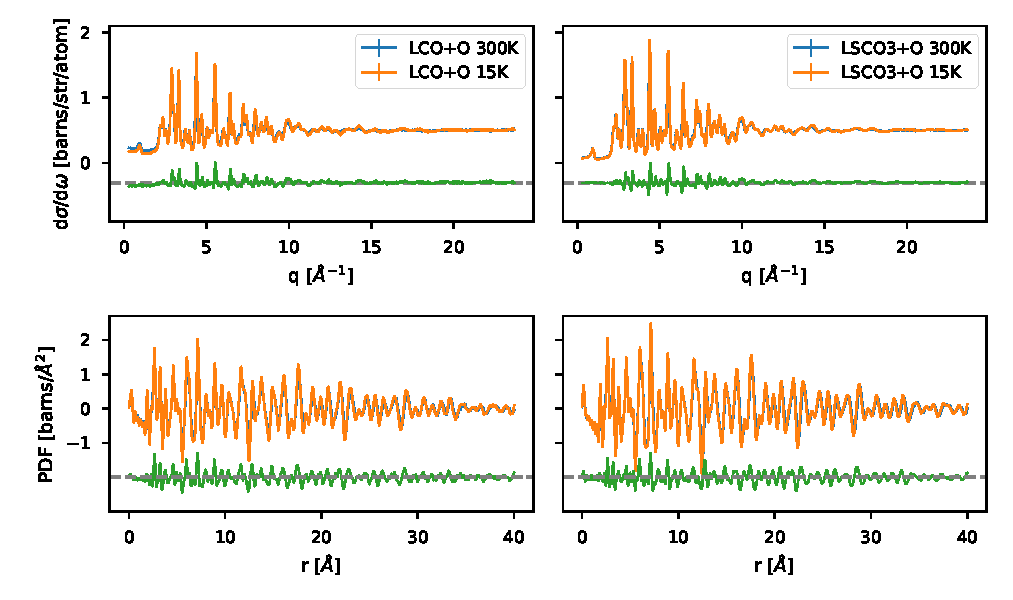
\includegraphics[width=\textwidth]{fig/pdf/temperature_comparison.pdf}
    \caption{Comparison of \SI{300}{\kelvin} and \SI{15}{\kelvin} for LCO+O and LSCO3+O in both real and reciprocal space.}
    \label{fig:temperature_comparision}    
\end{figure}

\begin{figure}[H]
    \centering
    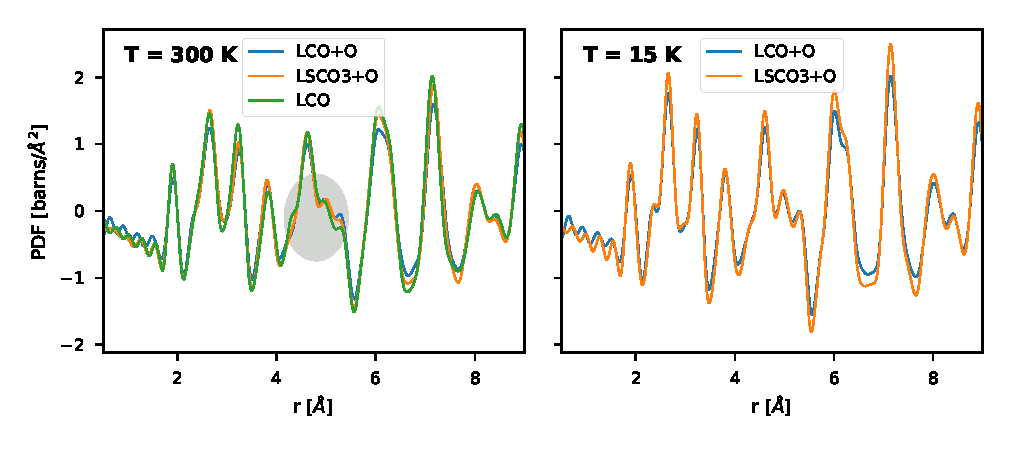
\includegraphics[width=\textwidth]{fig/pdf/medium_range_pdf.pdf}
    \caption{Short range PDF for all samples at \SI{300}{\kelvin} and \SI{15}{\kelvin}.}
    \label{fig:medium_range_pdf}    
\end{figure}

\begin{figure}[H]
    \centering
    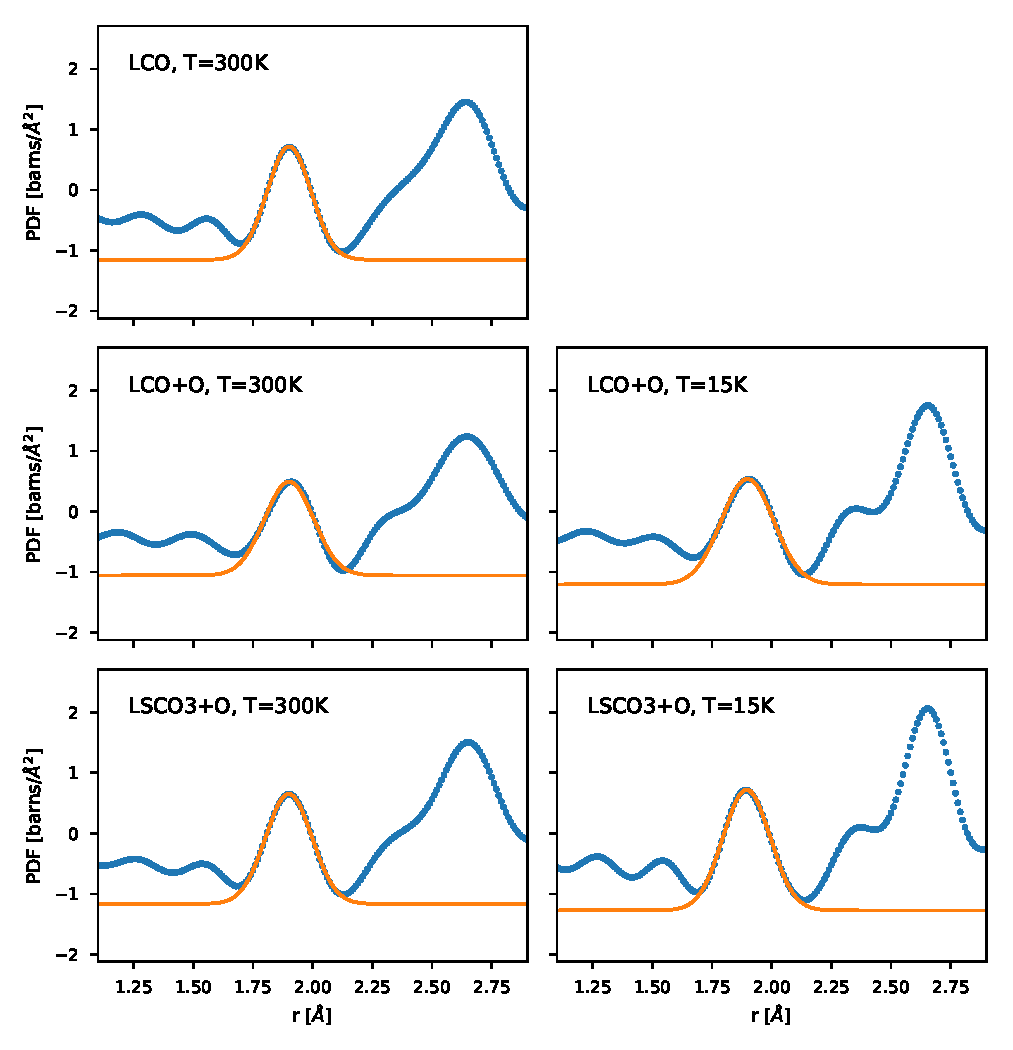
\includegraphics[width=\textwidth]{fig/pdf/cu_o_fits.pdf}
    \caption{Cu-O distance Gaussian fits.}
    \label{fig:cu_o_fits}
\end{figure}

\begin{table}[H]
    \centering
    \begin{tabular}{llll}
        \toprule
          Sample & Temperature [K] &        Cu-O distance [\AA] &           Cu-O $\sigma$ [\AA] \\
        \midrule
             LCO &         300 &  1.9010 $\pm$ 0.0003 &  0.0919 $\pm$ 0.0010 \\
           LCO+O &         300 &  1.9010 $\pm$ 0.0012 &  0.1024 $\pm$ 0.0054 \\
         LSCO3+O &         300 &  1.8995 $\pm$ 0.0003 &  0.0971 $\pm$ 0.0012 \\
           LCO+O &          15 &  1.8983 $\pm$ 0.0009 &  0.1099 $\pm$ 0.0048 \\
         LSCO3+O &          15 &  1.8945 $\pm$ 0.0003 &  0.0987 $\pm$ 0.0012 \\
        \bottomrule
    \end{tabular}    
    \caption{Cu-O distances in all samples at all available temperatures.}
    \label{tab:cu_o_fits}
\end{table}

\begin{figure}[]
    \centering
    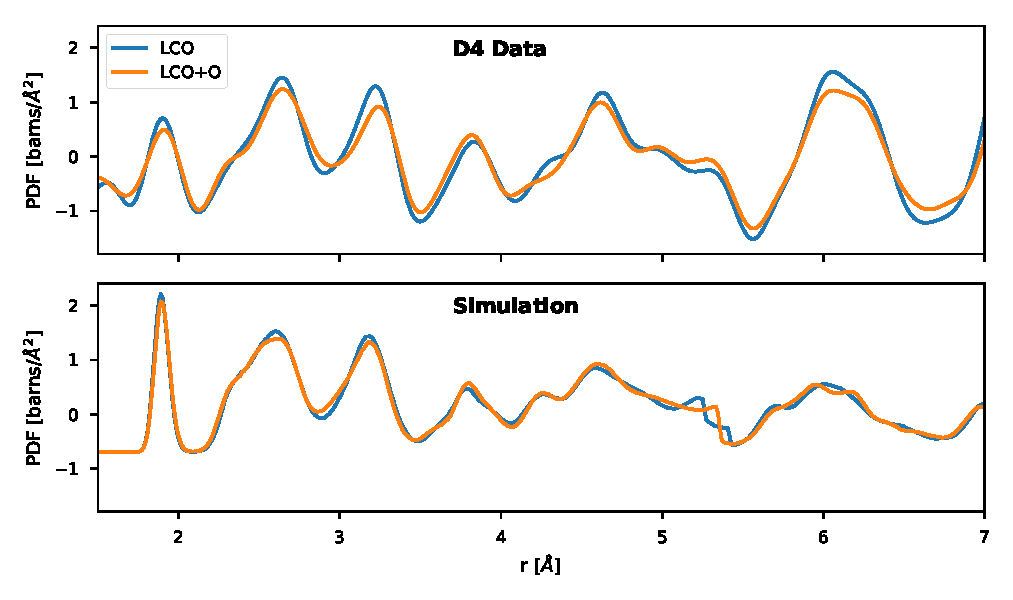
\includegraphics[width=\textwidth]{fig/pdf/pdf_simulation_experiment_compare.pdf}
    \caption[PDF data compared with MD simulation]{PDF data compared with MD simulation}
    \label{fig:pdf_sim_comparision}
\end{figure}